\subsection{BÀI TẬP TỰ LUYỆN}
\ind{PHẦN I.} \inden{Câu trắc nghiệm nhiều phương án lựa chọn. Mỗi câu hỏi học sinh chỉ chọn một phương án.}\\
\setcounter{ex}{0}
\Opensolutionfile{ans}[ans/0H4-B1-1]


\begin{ex}%[0H1Y1-1]
	Vectơ có điểm đầu $ M $ và điểm cuối $ N $ được kí hiệu như thế nào là đúng?
	\choice
	{$ MN $}
	{$ NM $}
	{\True $ \overrightarrow{MN} $}
	{$ \overrightarrow{mn}$}
	\loigiai{Vectơ có điểm đầu $ M $ và điểm cuối $ N $ được kí hiệu $ \overrightarrow{MN} $.
	}
\end{ex}

\begin{ex}%[0H1B1-1]
	Cho hai điểm phân biệt $ A $, $ B $. Số vectơ (khác $ \overrightarrow{0} $) có điểm đầu và điểm cuối lấy từ các điểm $ A $, $ B $ là
	\choice
	{\True $ 2 $}
	{$ 6 $}
	{$ 13 $}
	{$ 12 $}
	\loigiai{Có 2 vectơ có điểm đầu và điểm cuối lấy từ các điểm $ A $, $ B $ là $ \overrightarrow{AB} $ và $ \overrightarrow{BA} $.
	}
\end{ex}

\begin{ex}%[0H1Y1-3]
	Khẳng định nào sau đây đúng?
	\choice
	{Hai vectơ được gọi là bằng nhau nếu chúng cùng phương và cùng độ dài}
	{\True Hai vectơ được gọi là bằng nhau nếu chúng cùng hướng và cùng độ dài}
	{Hai vectơ được gọi là bằng nhau nếu chúng cùng hướng}
	{Hai vectơ được gọi là bằng nhau nếu chúng cùng độ dài}
	\loigiai{
		Theo khái niệm \lq\lq hai vectơ bằng nhau\rq\rq.\
	}
\end{ex}

\begin{ex}%[0H1Y1-2]
	Cho ba điểm $A, B, C$ thẳng hàng theo thứ tự đó. Cặp vectơ nào sau đây cùng hướng?
	\choice
	{$\overrightarrow{AC}$ và $\overrightarrow{CB}$}
	{$\overrightarrow{AB}$ và $\overrightarrow{CB}$}
	{$\overrightarrow{BA}$ và $\overrightarrow{BC}$}
	{\True $\overrightarrow{AB}$ và $\overrightarrow{BC}$}
	\loigiai{
		Ta có $A, B, C$ thẳng hàng và $B$ ở giữa $A, C$ nên ta có $\overrightarrow{AB}$ và $\overrightarrow{BC}$ cùng hướng.}
\end{ex}

\begin{ex}%[0H1B1-2]
	Cho ba điểm phân biệt $A$, $B$, $C$ thẳng hàng theo thứ tự đó. Khẳng định nào sau đây là \textbf{sai}?
	\choice
	{$\overrightarrow{BC}$ ngược hướng với $\overrightarrow{BA}$}
	{$\overrightarrow{AB}$ cùng hướng với $\overrightarrow{BC}$}
	{$\overrightarrow{AC}$ cùng hướng với $\overrightarrow{BC}$}
	{\True $\overrightarrow{CB}$ ngược hướng với $\overrightarrow{BA}$}
	\loigiai{
		\begin{center}
			\begin{tikzpicture}[scale=1, line join=round, line cap=round]
				\tkzDefPoints{0/0/A,3/0/B, 5/0/C}
				\draw[->] (C)--(B);
				\draw[->] (B)--(A);
				\tkzLabelPoints[below](A)
				\tkzLabelPoints[below](B)
				\tkzLabelPoints[below](C)
				\tkzDrawPoints[size=3,fill=black](A,B,C)
			\end{tikzpicture}
		\end{center}
		Dễ thấy $\overrightarrow{CB}$ cùng hướng với $\overrightarrow{BA}$.}
\end{ex}

\begin{ex}%[0H1B1-2]
	\immini[thm]{Cho hình bình hành $ABCD$ tâm $O$. Trên hình vẽ, số vectơ (khác $\overrightarrow{0}$, khác $\overrightarrow{AC}$) cùng phương với vectơ $\overrightarrow{AC}$ là
		\choice
		{$2$}
		{$3$}
		{$4$}
		{\True $5$}}{
		\begin{tikzpicture}[scale=1,font=
			\footnotesize,line join=round,line cap=round, >=stealth]
			\tkzDefPoints{0/0/A,4/0/B,5/1.5/C}
			\tkzDefPointBy[translation = from B to A](C)  \tkzGetPoint{D}
			\tkzInterLL(A,C)(B,D)    \tkzGetPoint{O}
			\tkzDrawSegments(A,B B,C C,D D,A A,C B,D)
			\tkzDrawPoints[size=2](A,B,C,D,O)
			\tkzLabelPoints[left](A,D)
			\tkzLabelPoints[right](C,B)
			\tkzLabelPoints[above](O)
	\end{tikzpicture}}
	\loigiai{
		\immini{Các vectơ (khác $\overrightarrow{0}$, khác $\overrightarrow{AC}$) cùng phương với $\overrightarrow{AC}$ là: $$\overrightarrow{AO}, \overrightarrow{OA}, \overrightarrow{CO}, \overrightarrow{OC}, \overrightarrow{CA}.$$}
		{\begin{tikzpicture}[scale=1,font=
				\footnotesize,line join=round,line cap=round, >=stealth]
				\tkzDefPoints{0/0/A,4/0/B,5/1.5/C}
				\tkzDefPointBy[translation = from B to A](C)  \tkzGetPoint{D}
				\tkzInterLL(A,C)(B,D)    \tkzGetPoint{O}
				\tkzDrawSegments(A,B B,C C,D D,A A,C B,D)
				\tkzDrawPoints(A,B,C,D,O)
				\tkzLabelPoints[left](A,D)
				\tkzLabelPoints[right](C,B)
				\tkzLabelPoints[above](O)
		\end{tikzpicture}}
	}
\end{ex}

\begin{ex}%[0H1B1-3]
	Gọi $M$ là trung điểm của đoạn thẳng $AB$. Khẳng định nào sau đây là đúng?
	\choice
	{\True $\overrightarrow{AB}$ và $\overrightarrow{AM}$ cùng phương}
	{$\overrightarrow{MA}=\overrightarrow{MB}$}
	{$\left|\overrightarrow{AB}\right|=\left|\overrightarrow{MB}\right|$}
	{$\overrightarrow{AB}$ và $\overrightarrow{MB}$ ngược hướng}
	\loigiai{
		Do $M$ là trung điểm của đoạn thẳng $AB$ nên $\overrightarrow{AB}$ và $\overrightarrow{AM}$ cùng phương.}
\end{ex}

\begin{ex}%[0H1B1-3]
	Cho tam giác đều $ABC$, mệnh đề nào sau đây là mệnh đề \textbf{sai}?
	\choice
	{$\overrightarrow{AC}$ không cùng phương $\overrightarrow{BC}$}
	{\True $\overrightarrow{AB}=\overrightarrow{BC}$}
	{$\overrightarrow{AC}\ne\overrightarrow{BC}$}
	{$\left|\overrightarrow{AB}\right|=\left|\overrightarrow{BC}\right|$}
	\loigiai{
		\immini{Hai vectơ $\overrightarrow{AB}, \overrightarrow{BC}$ không cùng hướng nên chúng không bằng nhau.}
		{\begin{tikzpicture}[scale=0.5, line join=round, line cap=round]
				\tkzDefPoints{0/0/A,4/0/B, 2/3/C}
				\tkzDrawSegments(C,A)
				\draw[->] (A)--(B);
				\draw[->] (B)--(C);
				\tkzLabelPoints[above](C)
				\tkzLabelPoints[left](A)
				\tkzLabelPoints[right](B)
				\tkzDrawPoints[size=3,fill=black](A,B,C)
		\end{tikzpicture}}
	}
\end{ex}

\begin{ex}%[0H1B1-3]
	Cho hình chữ nhật $ABCD$ có tâm là $I$. Khẳng định nào sau đây là đúng?
	\choice
	{$\overrightarrow{IC}=\overrightarrow{DI}$}
	{\True $\overrightarrow{AI}=\overrightarrow{IC}$}
	{$\overrightarrow{BI}=\overrightarrow{DI}$}
	{$\overrightarrow{IA}=\overrightarrow{BI}$}
	\loigiai{
		\immini{Do $I$ là tâm của hình chữ nhật $ABCD$ nên $I$ là trung điểm của $AC$.\\Vậy ta có $\overrightarrow{AI}=\overrightarrow{IC}$.}
		{\begin{tikzpicture}[scale=1, line join=round, line cap=round]
				\tkzDefPoints{0/0/A,3/0/B}
				\tkzDefGoldRectangle(A,B)
				\tkzGetPoints{C}{D}
				\tkzDrawPolygon(A,B,C,D)
				\tkzDrawSegments(A,C B,D)
				\tkzDefMidPoint(A,C)
				\tkzGetPoint{I}
				\draw[->] (A)--(I);
				\draw[->] (I)--(C);
				\tkzDrawPoints[fill=black,size=4](D,C,A,B,I)
				\tkzLabelPoints[below](A,B,I)
				\tkzLabelPoints[above](C,D)
		\end{tikzpicture}}
	}
\end{ex}

\begin{ex}%[0H1K1-3]
	Cho tứ giác $ABCD$ có $\overrightarrow{AB}=\overrightarrow{DC}$ và $\left|\overrightarrow{AB}\right|=\left|\overrightarrow{AD}\right|$ thì tứ giác $ABCD$ là hình gì?
	\choice
	{Hình bình hành}
	{\True Hình thoi}
	{Hình chữ nhật}
	{Hình vuông}
	\loigiai{
		\immini{Do $\overrightarrow{AB}=\overrightarrow{DC}$ nên $ABCD$ là hình bình hành.\\Mặt khác $\left|\overrightarrow{AB}\right|=\left|\overrightarrow{AD}\right|$ nên $ABCD$ là hình thoi.}{\begin{tikzpicture}[scale=0.5, line join=round, line cap=round]
				\tkzDefPoints{0/0/A,3/2/B,6/0/C,3/-2/D}
				\tkzDrawSegments(A,B B,C C,D D,A)
				\tkzLabelPoints[left](A)
				\tkzLabelPoints[above](B)
				\tkzLabelPoints[right](C)
				\tkzLabelPoints[below](D)
				\tkzDrawPoints[size=3,fill=black](A,B,C,D)
		\end{tikzpicture}}
	}
\end{ex}

\begin{ex}%[0H1B1-2]
	Cho tứ giác $A$, $B$, $C$, $D$ thỏa mãn $\overrightarrow{AB}=\overrightarrow{DC}$, phát biểu nào sau đây là \textbf{sai}?
	\choice
	{$AB=CD$}
	{\True  $\overrightarrow{AB}$ và $\overrightarrow{CD}$ là hai vectơ cùng hướng}
	{$AC$ và $BD$ nhận cùng một điểm làm trung điểm}
	{$ABCD$ là hình bình hành}
	\loigiai{
		$ABCD$ là hình bình hành khi bốn điểm $A$, $B$, $C$, $D$ không thẳng hàng.}
\end{ex}

\begin{ex}%[0H1B1-2]
	Cho tam giác $ABC$, gọi $M$, $N$ lần lượt là trung điểm của hai cạnh $AB$ và $AC$. Mệnh đề nào dưới đây đúng?
	\choice
	{$\overrightarrow{MN}$ và $\overrightarrow{AC}$ cùng phương}
	{\True $\overrightarrow{MN}$ và $\overrightarrow{BC}$ cùng phương}
	{$\overrightarrow{MN}$ và $\overrightarrow{AB}$ cùng phương}
	{$\overrightarrow{MN}$ và $\overrightarrow{BN}$ cùng phương}
	\loigiai{
		\immini{
			Ta có $MN$ là đường trung bình của tam giác $ABC$ nên $MN\parallel BC$. Do đó hai vectơ $\overrightarrow{MN}$ và $\overrightarrow{BC}$ cùng phương.
		}
		{
			\begin{tikzpicture}[scale=1,font=\footnotesize,line join=round, line cap=round,>=stealth]
				\tkzDefPoints{2/3/A,0/0/B,5/0/C}
				\tkzDefMidPoint(A,B)\tkzGetPoint{M}
				\tkzDefMidPoint(A,C)\tkzGetPoint{N}
				\tkzDrawPoints[fill=black](A,B,C,N,M)
				\tkzDrawSegments(M,N)
				\tkzDrawPolygon(A,B,C)
				\tkzLabelPoints[left](B,M)
				\tkzLabelPoints[above](A)
				\tkzLabelPoints[right](C,N)
			\end{tikzpicture}
		}
	}
\end{ex}

\begin{ex}
	\immini[thm]{Cho hình bình hành $ABCD$ tâm $O$. Khẳng định nào sau đây là đúng?
		\choice
		{$\overrightarrow{AB}=\overrightarrow{CD}$}
		{$\overrightarrow{OA}=\overrightarrow{OC}$}
		{$\overrightarrow{OB}=\overrightarrow{OD}$}
		{\True $\overrightarrow{AD}=\overrightarrow{BC}$}
	}{\hspace{1cm}
		\begin{tikzpicture}[scale=1, line join=round, line cap=round]
			\tkzDefPoints{0/0/A,4/0/B,5/2/C}
			\tkzDefPointBy[translation=from B to C](A)\tkzGetPoint{D}
			\tkzInterLL(A,C)(B,D)\tkzGetPoint{O}
			\tkzDrawSegments(A,B B,C C,D D,A A,C B,D)
			\tkzDrawPoints[size=3,fill=black](A,B,C,D,O)
			\tkzLabelPoints[below,font=\footnotesize](A, B, O)
			\tkzLabelPoints[above,font=\footnotesize](C,D)
	\end{tikzpicture}}
\end{ex}

\begin{ex}%[0H1B1-2]
	Cho hình bình hành $ABCD$. Hai vectơ nào ngược hướng?
	\choice
	{$\overrightarrow{AB}$ và $\overrightarrow{DB}$}
	{$\overrightarrow{AB}$ và $\overrightarrow{AC}$}
	{\True $\overrightarrow{AB}$ và $\overrightarrow{CD}$}
	{$\overrightarrow{AB}$ và $\overrightarrow{DC}$}
	\loigiai{
		\begin{center}
			\begin{tikzpicture}[>=stealth, line join = round, line  cap = round,scale=1]
				\tkzDefPoints{2/2/A,0/0/B,4/0/C}
				\tkzDefPointBy[translation=from B to C](A) \tkzGetPoint{D}
				\tkzDrawSegments(A,B B,C C,D D,A)
				\tkzDrawPoints[fill,size=2](A,B,C,D)
				\tkzLabelPoints[below](B,C)
				\tkzLabelPoints[above](A,D)
			\end{tikzpicture}
		\end{center}
		Hai vectơ $\overrightarrow{AB}$ và $\overrightarrow{CD}$ ngược hướng.
	}
\end{ex}

\begin{ex}%[0H1B1-3]
	\immini[thm]{Cho tam giác đều $ABC$ cạnh $a$, có trung tuyến $BM$. Độ dài của $\overrightarrow{BM}$ là
		\haicot
		{$a\sqrt{3}$}
		{$\dfrac{a\sqrt{2}}{3}$}
		{\True $\dfrac{a\sqrt{3}}{2}$}
		{$\dfrac{a\sqrt{3}}{3}$}}{
		\begin{tikzpicture}[smooth,font=\footnotesize,scale=0.8]
			\path
			(0,0) coordinate (B)
			(4,0) coordinate (C)
			($(B)!1!60:(C)$)coordinate (A)
			($(A)!0.5!(C)$)coordinate (M);
			\draw (A)--(B)--(C)--cycle (B)--(M);
			\foreach \x/\g in {A/90,B/-90,C/-90,M/0} \draw [fill=black] (\x) circle (.05) + (\g:.3) node{$\x$};
	\end{tikzpicture}}
	\loigiai{
		Trong tam giác đều $ABC$ cạnh $a$, có trung tuyến $BM=\left|\overrightarrow{BM}\right|=\dfrac{a\sqrt{3}}{2}$.}
\end{ex}

\begin{ex} 
	\immini[thm]{Cho hình vuông $ABCD$ cạnh bằng $a$. Gọi $M$ là trung điểm của $CD$. Tính độ lớn của vectơ $\overrightarrow{AM}$.
		\haicot
		{ $\dfrac{a\sqrt{3}}{2}$}
		{\True $\dfrac{a\sqrt{5}}{2}$}
		{ $\dfrac{3a}{2}$}
		{ $\dfrac{5a}{2}$}
	}{
		\begin{tikzpicture}[scale=1, line join=round, line cap=round]
			\tkzDefPoints{0/0/A,3/0/B,3/3/C}
			\coordinate (D) at ($(A)+(C)-(B)$);
			\coordinate (M) at ($(C)!0.5!(D)$);
			\tkzDrawSegments(A,B B,C C,D D,A A,M)
			\tkzDrawPoints[size=3,fill=black](A,B,C,D,M)
			\tkzLabelPoints[below](A,B)
			\tkzLabelPoints[above](C,D,M)
	\end{tikzpicture}}
	\loigiai{
	Vì $ABCD$ là hình vuông cạnh $a$ và $M$ là trung điểm của $CD$ nên $DM = \dfrac{a}{2}$.\\
	Xét tam giác $ADM$ vuông tại $D$, áp dụng định lý Pythagore ta có:
	$$ AM = \sqrt{AD^2 + DM^2} = \sqrt{a^2 + \left(\dfrac{a}{2}\right)^2} = \sqrt{\dfrac{5a^2}{4}} = \dfrac{a\sqrt{5}}{2}. $$
	Độ lớn của vectơ $\overrightarrow{AM}$ là $|\overrightarrow{AM}| = AM = \dfrac{a\sqrt{5}}{2}$.
}
\end{ex}

\Closesolutionfile{ans}

\ind{PHẦN II.} \inden{Câu trắc nghiệm đúng sai. Trong mỗi ý a), b), c), d) ở mỗi câu, học sinh chọn đúng hoặc sai.}\\
\Opensolutionfile{ans}[ans/0H4-B1-2]

\begin{ex}
	Gọi ${K}$ là trung điểm của đoạn thẳng ${PQ}$. Xét tính đúng sai của các khẳng định sau:
	\choiceTF
	{ \True $\overrightarrow{QP}$ và $\overrightarrow{QK}$ là cùng phương }
	{ $\overrightarrow{KP}=\overrightarrow{KQ}$ }
	{ $|\overrightarrow{QP}|=|\overrightarrow{QK}|$ }
	{ $\overrightarrow{QP}$ và $\overrightarrow{QK}$ là ngược hướng }
	\loigiai{
	\begin{itemchoice}
		\itemch Đúng. Ba điểm $Q, K, P$ thẳng hàng nên hai vectơ $\overrightarrow{QP}$ và $\overrightarrow{QK}$ cùng phương (thực chất là cùng hướng).
		\itemch Sai. $K$ là trung điểm của $PQ$ nên $\overrightarrow{KP}$ và $\overrightarrow{KQ}$ là hai vectơ đối nhau, suy ra $\overrightarrow{KP} = -\overrightarrow{KQ}$.
		\itemch Sai. $K$ là trung điểm của $PQ$ nên $QP = 2QK$, do đó $|\overrightarrow{QP}| = 2|\overrightarrow{QK}|$.
		\itemch Sai. Vì $K$ nằm giữa $Q$ và $P$ nên hai tia $QP$ và $QK$ trùng nhau, suy ra $\overrightarrow{QP}$ và $\overrightarrow{QK}$ cùng hướng.
	\end{itemchoice}
}
\end{ex}

\begin{ex}
	\immini[thm]{Cho hình bình hành ${ABCD}$ tâm $O$. Xét tính đúng sai của các khẳng định sau:
	\choiceTF
	{\True $\overrightarrow{DA}$ và $\overrightarrow{CB}$ là cùng hướng }
	{$\vec{OA}=\vec{OC}$}
	{\True $|\overrightarrow{OB}|=|\overrightarrow{OD}|$}
	{$|\overrightarrow{AC}|=|\overrightarrow{BD}|$}
}{
\begin{tikzpicture}[scale=0.9, font=\footnotesize,>=stealth]
	\path
	%	Vẽ mp
	(0,0) coordinate (A)
	(3,0) coordinate (B)
	(4,1.5) coordinate (C)
	($(A)+(C)-(B)$)coordinate (D)
	;
	\draw (A)--(B)--(C)--(D)--(A) (B)--(D) (A)--(C);
	\foreach \x/\g in {A/180,B/0,C/0,D/180}\draw[fill=black] (\x) circle (.05) +(\g:.5)node{\footnotesize$\x$};
\end{tikzpicture}}
	\loigiai{
	\begin{itemchoice}
		\itemch Đúng. Vì $ABCD$ là hình bình hành nên $AD \parallel BC$ và $AD = BC$. Mặt khác, hướng từ $D$ đến $A$ và từ $C$ đến $B$ là giống nhau nên $\overrightarrow{DA}$ và $\overrightarrow{CB}$ cùng hướng (và bằng nhau).
		\itemch Sai. $O$ là tâm hình bình hành nên $O$ là trung điểm của $AC$. Hai vectơ $\overrightarrow{OA}$ và $\overrightarrow{OC}$ ngược hướng nên $\overrightarrow{OA} = -\overrightarrow{OC}$.
		\itemch Đúng. $O$ là trung điểm của đường chéo $BD$ nên $OB = OD \Rightarrow |\overrightarrow{OB}| = |\overrightarrow{OD}|$.
		\itemch Sai. Độ dài hai đường chéo của hình bình hành nói chung không bằng nhau ($AC \neq BD$).
	\end{itemchoice}
}\end{ex}

\begin{ex}
	\immini[thm]{Cho tam giác đều ${DEF}$. Gọi $M$ là trung điểm của đoạn $DE$. Xét tính đúng sai của các khẳng định sau:
	\choiceTF
	{$\overrightarrow{DE}=\overrightarrow{DF}$ }
	{$\vec{ME}=\vec{MD}$}
	{\True $\vec{ME}$ cùng phương với $\vec{ED}$}
	{ \True $|\overrightarrow{ED}|=|\overrightarrow{EF}|$ }}{
		\begin{tikzpicture}[scale=0.7, font=\footnotesize,>=stealth]
		\path
		%	Vẽ mp
		(0,0) coordinate (D)
		(3,0) coordinate (E)
		($(D)!1!60:(E)$)coordinate (F)
		;
		\draw (D)--(E)--(F)--(D);
		\foreach \x/\g in {D/180,E/0,F/90}\draw[fill=black] (\x) circle (.05) +(\g:.4)node{\footnotesize$\x$};
\end{tikzpicture}}
	\loigiai{
	\begin{itemchoice}
		\itemch Sai. Hai vectơ $\overrightarrow{DE}$ và $\overrightarrow{DF}$ có hướng khác nhau nên không thể bằng nhau.
		\itemch Sai. $M$ là trung điểm của $DE$ nên $\overrightarrow{ME}$ và $\overrightarrow{MD}$ là hai vectơ đối nhau ($\overrightarrow{ME} = -\overrightarrow{MD}$).
		\itemch Đúng. Ba điểm $E, M, D$ cùng nằm trên một đường thẳng nên các vectơ tạo thành từ ba điểm này đều cùng phương.
		\itemch Đúng. Vì tam giác $DEF$ đều nên $ED = EF \Rightarrow |\overrightarrow{ED}| = |\overrightarrow{EF}|$.
	\end{itemchoice}
}
\end{ex}

\begin{ex}
	\immini[thm]{Cho hình vuông ${ABCD}$ cạnh bằng $a$, $I$ là điểm trên cạnh $BC$ thỏa $CI=\dfrac{1}{2}IB$. Xét tính đúng sai của các khẳng định sau: 
	\choiceTF
	{\True $\overrightarrow{DA}$ và $\overrightarrow{BC}$ là ngược hướng }
	{ $\overrightarrow{AC}=\overrightarrow{BD}$ }
	{$\big|\overrightarrow{AC}\big|=2a$}
	{\True $\big|\overrightarrow{AI}\big|=\dfrac{\sqrt{13}a}{3}$}}{\hspace{1cm}
		\begin{tikzpicture}[scale=0.7, font=\footnotesize,>=stealth]
		\path
		%	Vẽ mp
		(0,0) coordinate (A)
		(3,0) coordinate (B)
		($(A)!1!90:(B)$)coordinate (D)
		($(B)!1!-90:(A)$)coordinate (C)
		;
		\draw (A)--(B)--(C)--(D)--(A);
		\foreach \x/\g in {A/180,B/0,C/0,D/180}\draw[fill=black] (\x) circle (.05) +(\g:.4)node{\footnotesize$\x$};
\end{tikzpicture}}
	\loigiai{
	\begin{itemchoice}
		\itemch Đúng. Trong hình vuông $ABCD$, $\overrightarrow{AD}$ và $\overrightarrow{BC}$ là hai vectơ bằng nhau (cùng hướng, cùng độ dài). Suy ra $\overrightarrow{DA}$ (vectơ đối của $\overrightarrow{AD}$) sẽ ngược hướng với $\overrightarrow{BC}$.
		\itemch Sai. Hai đường chéo $AC$ và $BD$ có phương cắt nhau nên hai vectơ $\overrightarrow{AC}$ và $\overrightarrow{BD}$ không cùng phương, do đó không thể bằng nhau.
		\itemch Sai. Đường chéo của hình vuông cạnh $a$ có độ dài là $a\sqrt{2}$. Vậy $|\overrightarrow{AC}| = a\sqrt{2}$.
		\itemch Đúng. Theo giả thiết $I \in BC$ và $CI = \dfrac{1}{2}IB \Rightarrow IB = \dfrac{2}{3}BC = \dfrac{2a}{3}$.\\
		Xét tam giác $ABI$ vuông tại $B$, áp dụng định lý Pythagore:
		$$ AI = \sqrt{AB^2 + IB^2} = \sqrt{a^2 + \left(\dfrac{2a}{3}\right)^2} = \sqrt{a^2 + \dfrac{4a^2}{9}} = \sqrt{\dfrac{13a^2}{9}} = \dfrac{a\sqrt{13}}{3}. $$
		Vậy $|\overrightarrow{AI}| = AI = \dfrac{\sqrt{13}a}{3}$.
	\end{itemchoice}
}\end{ex}


\Closesolutionfile{ans}

\ind{PHẦN III.} \inden{Câu trắc nghiệm trả lời ngắn.}\\
\Opensolutionfile{ans}[ans/0H4-B1-3]
\begin{ex}%[0H1B1-2]
	Cho các vectơ như hình vẽ. Có bao nhiêu cặp vectơ cùng phương xuất hiện trong hình?\\
	\shortans[oly]{$8$}
	\begin{center}
		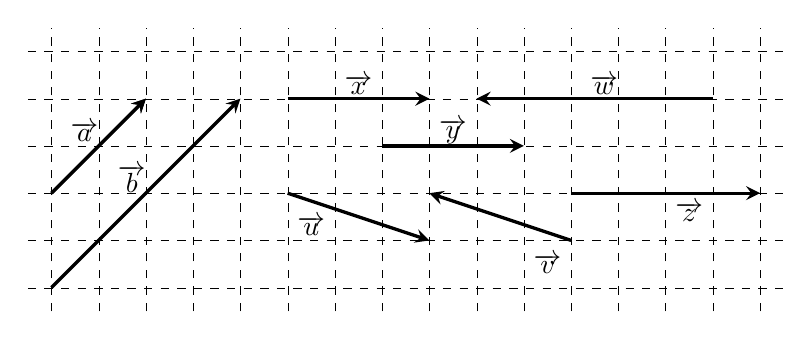
\begin{tikzpicture}[line width=1.2,>=stealth,scale=0.6]
			\draw[step=1,ultra thin,dashed](-0.5,-0.5)grid(15.5,5.5);
			\draw[->](0,2)--(2,4);
			\draw[->](0,0)--(4,4);
			\draw[->](5,4)--(8,4);
			\draw[->](5,2)--(8,1);
			\draw[->](7,3)--(10,3);
			\draw[->](0,2)--(2,4);
			\draw[->](14,4)--(9,4);
			\draw[->](11,2)--(15,2);
			\draw[->](11,1)--(8,2);
			\node at (0.7,3.3) {$\overrightarrow{a}$};
			\node at (1.7,2.3) {$\overrightarrow{b}$};
			\node at (5.5,1.3) {$\overrightarrow{u}$};
			\node at (10.5,0.5) {$\overrightarrow{v}$};
			\node at (13.5,1.6) {$\overrightarrow{z}$};
			\node at (6.5,4.3) {$\overrightarrow{x}$};
			\node at (8.5,3.3) {$\overrightarrow{y}$};
			\node at (11.7,4.3) {$\overrightarrow{w}$};
		\end{tikzpicture}
	\end{center}
	\loigiai{
		Có $8$ cặp vectơ cùng phương xuất hiện trong hình gồm: $\overrightarrow{a}$ và $\overrightarrow{b}$, $\overrightarrow{x}$ và $\overrightarrow{y}$, $\overrightarrow{x}$ và $\overrightarrow{z}$, $\overrightarrow{x}$ và $\overrightarrow{w}$, $\overrightarrow{y}$ và $\overrightarrow{z}$, $\overrightarrow{y}$ và $\overrightarrow{w}$, $\overrightarrow{z}$ và $\overrightarrow{w}$, $\overrightarrow{u}$ và $\overrightarrow{v}$.}
\end{ex}

\begin{ex}
	Cho hình vuông $ABCD$ có độ dài cạnh bằng $3$ cm. Tính độ dài  vectơ $\overrightarrow{AC}$. (kết quả làm tròn đến hai chữ số thập phân)\\
	\shortans[oly]{$4,24$}
	\loigiai{
		\immini{
			$\left|\overrightarrow{AC}\right|=AC=\sqrt{AB^2+BC^2}=\sqrt{3^2+3^2}=3\sqrt{2} \approx 4,24$ cm.
		}{
			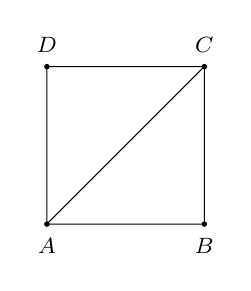
\begin{tikzpicture}[scale=1, font=\footnotesize, line join=round, line cap=round,>=stealth]
				\draw (0,0) rectangle (2,2) (0,0)--(2,2);
				\foreach\i/\j/\goc/\diem in{0/0/-90/A,2/0/-90/B,2/2/90/C,0/2/90/D}
				\fill(\i,\j) circle(1.0pt) node[shift={(\goc:8pt)}]{$\diem$};
			\end{tikzpicture}
		}
	}
\end{ex}

\begin{ex}%[0H5H1-5]
	\immini{
		Cho hình chữ nhật $ABCD$ có cạnh $AB=3$, $BC=4$. Độ dài của vectơ $\overrightarrow{DB}$ bằng bao nhiêu?\\
		\shortans[oly]{$5$}
	}{
		\begin{tikzpicture}[scale=0.8, font=\footnotesize, line join=round, line cap=round, >=stealth]
			\path	(0,0) coordinate (A)++(0:3) coordinate (D)
			($(A)+(-90:2)$) coordinate (B)
			($(B)+(D)-(A)$) coordinate (C)
			;
			\draw (A)--(B)--(C)--(D)--(A);
			\foreach \x/\g in {A/130,D/60,C/-30,B/-150}  \fill (\x) circle (1pt)+(\g:.3)node[scale=0.8]{$\x$};	
		\end{tikzpicture}
	}
	\loigiai{
		Áp dụng định lí Pitago cho tam giác vuông $ABC$ ta có 
		\[ AC=\sqrt{AB^2+BC^2}=\sqrt{3^2+4^2}=5. \]
		Vì $ABCD$ là hình chữ nhật nên $\left|\overrightarrow{DB}\right|=\left|\overrightarrow{AC}\right|=AC=5$.
	}
\end{ex}

\begin{ex}%[0H1B1-3]
	Cho tam giác $ABC$ đều cạnh bằng $1$, trọng tâm $G$. Độ dài vectơ $\overrightarrow{AG}$ bằng bao nhiêu? (kết quả làm tròn đến hai chữ số thập phân)\\
	\shortans[oly]{$0,58$}
	\loigiai{
		\immini
		{
			Gọi $I$ là trung điểm của $BC \Rightarrow AI=\dfrac{\sqrt{3}}{2}$.\\
			Ta có $AG=\dfrac{2}{3}AI=\dfrac{2}{3} \cdot \dfrac{\sqrt{3}}{2}=\dfrac{\sqrt{3}}{3} \Rightarrow \left|\overrightarrow{AG}\right|=\dfrac{\sqrt{3}}{3}$.
		}
		{
			\begin{tikzpicture}[>=stealth,line cap=round,line join=round,scale=.6,font=\footnotesize]
				\tkzDefPoints{-2/-3/B,4/-3/C}
				\tkzDefPointBy[rotation = center B angle 60](C)    \tkzGetPoint{A}
				\coordinate (I) at ($(C)!0.5!(B)$);
				\tkzCentroid(A,B,C)    \tkzGetPoint{G}
				\tkzDrawPolygon(A,B,C)
				\tkzDrawPoints[fill=black](A,B,C,I,G)
				\tkzDrawSegments(G,I)
				\draw[blue,->](A)--(G);
				\tkzLabelPoints[left](G,B)
				\tkzLabelPoints[above](A)
				\tkzLabelPoints[below](I)
				\tkzLabelPoints[right](C)
			\end{tikzpicture}
		}
	}
\end{ex}

\begin{ex}%[0H5H1-5]
	Cho tam giác $ABC$ đều có cạnh bằng $8$. Gọi $G$ là trọng tâm tam giác $ABC$ và $I$ là trung điểm của $AG$. Độ dài của vectơ $\overrightarrow{AI}$ (làm tròn kết quả đến hàng phần trăm) bằng bao nhiêu?\\
	\shortans[oly]{$2{,}31$}
	\loigiai{
		\immini{
			Gọi $M$ là trung điểm của $BC$. Ta có
			\[\begin{array}{l} {\left|\overrightarrow{AG}\right|=AG=\dfrac{2}{3} AM=\dfrac{2}{3} \sqrt{AB^2-BM^2}=\dfrac{2}{3} \sqrt{8^2-\dfrac{8^2}{4}}=\dfrac{8\sqrt{3}}{3}} \\ {\left|\overrightarrow{AI}\right|=AI=\dfrac{AG}{2}=\dfrac{4\sqrt{3}}{3} \approx 2{,}31} \end{array}
			\]
		}{
			\begin{tikzpicture}[scale=1, font=\footnotesize, line join=round, line cap=round, >=stealth]
				\path	(0,0) coordinate (B)++(0:3) coordinate (C)
				($(B)+(60:3)$) coordinate (A)
				($(B)!1/2!(C)$) coordinate (M)
				($(A)!2/3!(M)$) coordinate (G)
				($(A)!1/2!(G)$) coordinate (I)
				;
				\draw (A)--(B)--(C)--(A)--(M);
				\foreach \x/\g in {A/90,B/-150,C/-30,I/0,G/0,M/-90}  \fill (\x) circle (1pt)+(\g:.3)node[scale=1]{$\x$};	
			\end{tikzpicture}
		}
	}
\end{ex}

\Closesolutionfile{ans}